% !TeX spellcheck = en_US


\chapter{Introduction}


\section{Biological Whiskers}

Over the past two decades, tactile perception has gained attention within robotics, a field traditionally dominated by visual sensing~\cite{s22072705}.
Tactile sensing provides distinct advantages, especially when visibility is limited, in low-light conditions, or when environments are narrow, cluttered, or visually obstructed.
Nature provides ample evidence of the effectiveness of tactile sensing and offers inspiration for the development of tactile sensors.

Some animals possess tactile sensory hairs known as whiskers or vibrissae, which complement their vision.
Whiskers enable them to interact effectively with their environment through non-intrusive mechanical contact.
\enquote{Traditionally, whiskers are associated with diverse survival skills, including tactile discrimination, distance assessment, food acquisition, gap crossing, and social interaction} note Ibarra-Castaneda et al.~\cite{IBARRACASTANEDA2022100034}.
For example, seals and sea lions use their whiskers for hunting in dark and turbid environments.
When prey swims nearby, the generated hydrodynamic vortices cause distinct, jerky deflections in the whiskers.
These deflections reveal the hydrodynamic trail left by the prey, allowing seals and sea lions to locate their prey effectively~\cite{muthuramalingam2018sealsealionwhiskers}.
Thus, whiskers function as passive sensors by responding directly to external excitation.

In contrast, some rodents such as rats and squirrels can move their whiskers actively, in rhythmic motions known as \textit{whisking}, enabling them to actively perceive their immediate surroundings and to distinguish surface textures.
Different textures produce unique slip-stick motion patterns and deflection magnitudes of whiskers, resulting in characteristic resonant vibrations that rodents interpret to identify surfaces and objects~\cite{wolfe2008texture}.

Rats particularly depend on whisker-based navigation when traversing confined spaces, such as tunnels or burrows.
Through coordinated whisking motions, rats efficiently detect the layout and contours of the environment, allowing them to move even in complete darkness~\cite{*}.

The anatomical structure and functional mechanisms of biological whiskers are depicted in Figure~\ref{fig:whisker-anatomy}.
Whiskers come in various shapes and sizes, and one animal can have multiple whiskers, each with a different length and taper.
Sensory detection is carried out solely by mechanoreceptors located at the base of each whisker follicle, without any additional receptors along the whisker shaft~\cite{doi:10.1089/soro.2016.0028}.
This simplicity, effectiveness and variability of biological whiskers provides a foundation for developing biomimetic tactile sensors.

\begin{figure}[htb]
    \centering
    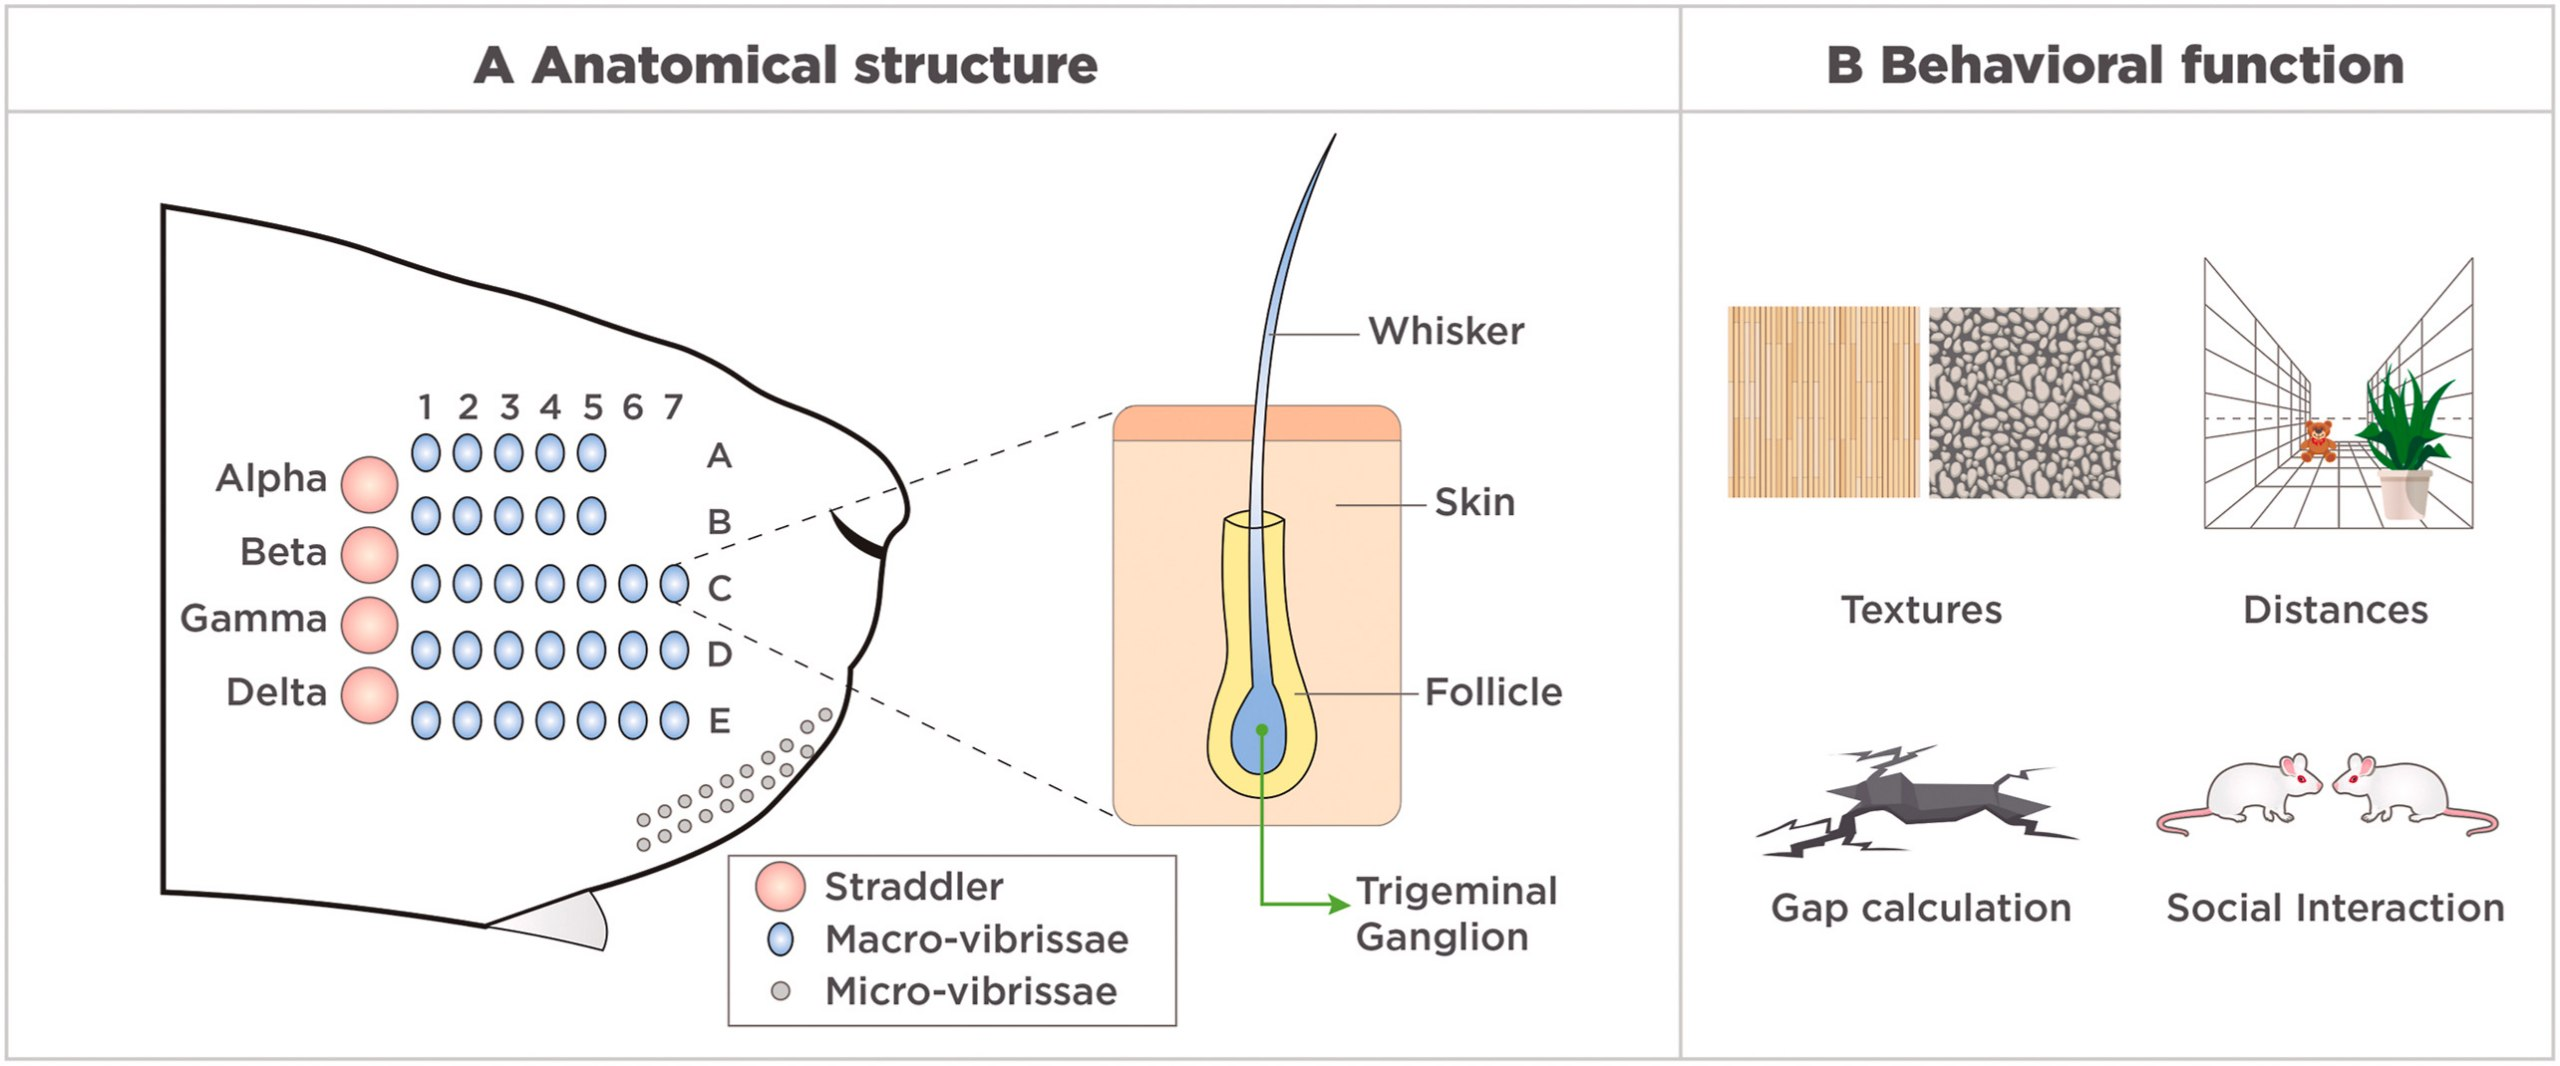
\includegraphics[width=\textwidth]{figures/whisker-anatomy}
    \caption{Representation of the vibrissae system and its function, from~\cite{IBARRACASTANEDA2022100034}}
    \label{fig:whisker-anatomy}
\end{figure}


\section{Whisker-inspired Tactile Sensors}

The versatility and effectiveness of biological whiskers have inspired numerous developments in the field.
Whisker-inspired tactile sensors have extensive applications, including~\cite{s22072705}:
\begin{itemize}
    \item Recognition of the surrounding objects and obstacle avoidance (extraction of the 3D whisker tip position)
    \item Exploration of unstructured environments
    \item Leak detection in pipelines
    \item Water flow detection in unmanned underwater vehicles
    \item Midair obstacle detection for drones
    \item Tactile sensing of heart valves
    \item Navigation in dark or visually obscured environments
    \item Study of the surface texture (like surface hardness and adhesiveness of food)~\cite{https://doi.org/10.1002/aisy.202300660}
\end{itemize}

Whisker-inspired tactile sensors offer low power consumption, minimal computational requirements, and high spatial resolution.
Some of the most commonly used whisker-inspired tactile sensors are:~\cite{s22072705}
\begin{itemize}
    \item \textbf{Strain gauge sensors:} measure changes in electrical resistance caused by deformation of strain gauges attached to the whisker shaft.
    \item \textbf{Hall effect sensors:} detect changes in magnetic field strength caused by displacement or rotation of the magnet positioned at the whisker base.
    \item \textbf{Capacitive sensors:} detect changes in capacitance caused by deformation of the whisker.
    \item \textbf{Piezoelectric sensors:} generate an electrical charge in response to mechanical stress applied to the whisker.
    \item \textbf{Optical sensors:} change light path or intensity as the fiber-based whisker deflects.
    \item \textbf{Magnetoresistive sensors:} measure changes in electrical resistance caused by changes in magnetic fields when whisker deflection occurs.
    \item \textbf{MEMS-based sensors:} employs a capacitive or piezoelectric sensor in a microelectromechanical system format.
\end{itemize}
Taxonomy of whisker sensors is shown in Figure~\ref{fig:taxonomy}.

\begin{figure}[htb]
    \centering
    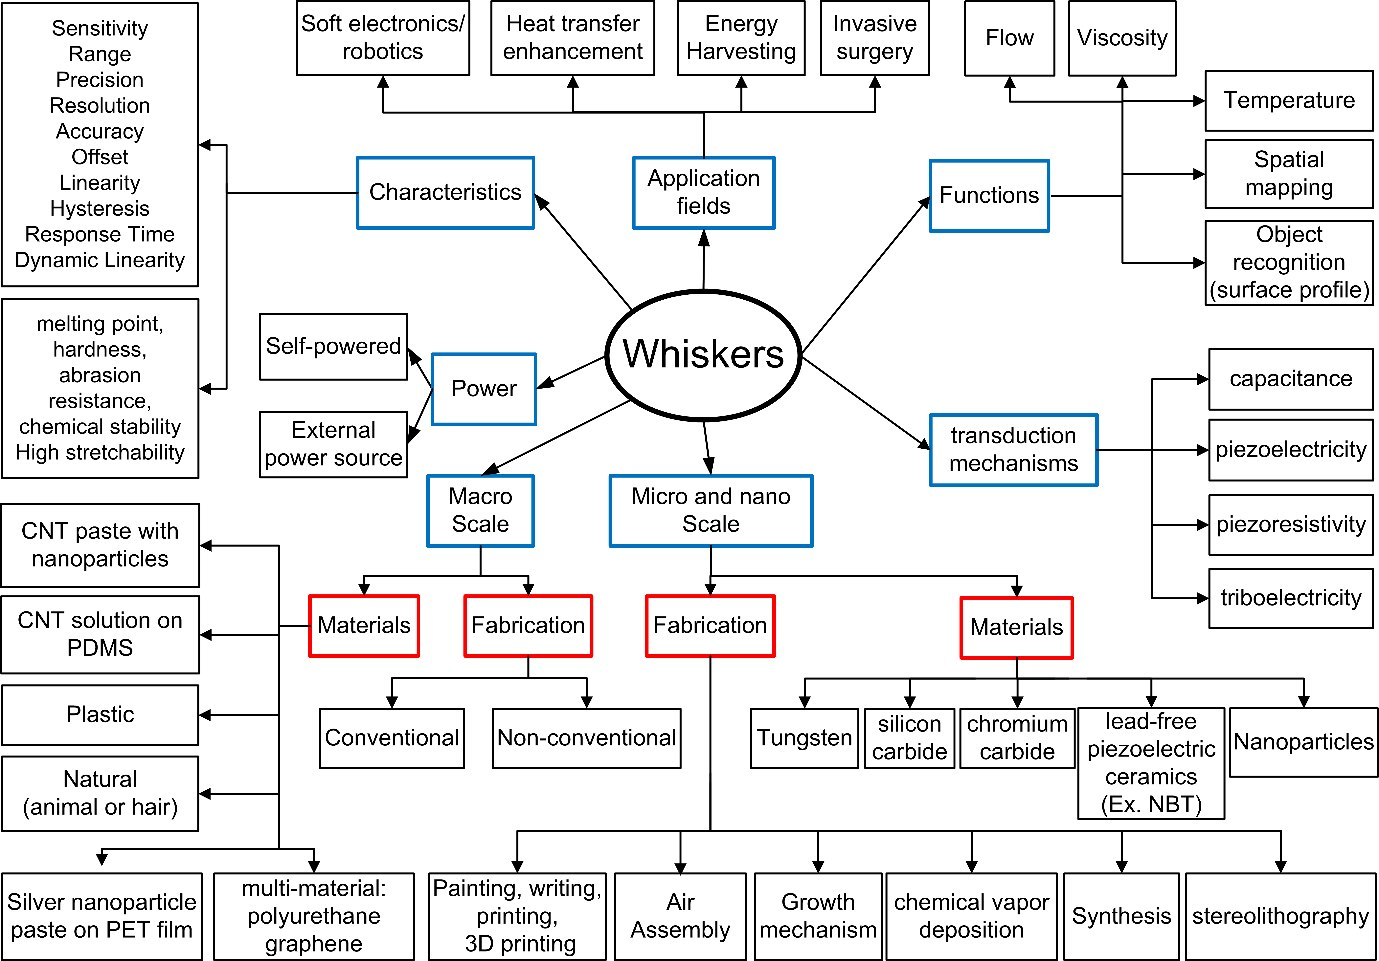
\includegraphics[width=0.65\textheight]{figures/taxonomy}
    \caption{A taxonomy for whisker-based sensors, from \cite{s22072705}}
    \label{fig:taxonomy}
\end{figure}


\section{Active Tactile Perception}
One of the most critical problems in robotics is \textbf{reconstruction of unstructured environments}.
It is essential for efforts to develop \textbf{autonomous mobile manipulators}, that are said to have significant societal and economic impact~\cite{how-can-robots-succeed}.
Operation in unstructured environments poses multiple challenges, such as:~\cite{how-can-robots-succeed}
\begin{itemize}
    \item Limited knowledge of the surroundings
    \item Uncertainty in the robot's position
    \item Constraints on the robot's mobility
    \item Impermanence of the state of the environment
\end{itemize}
Thus, the reconstruction of unstructured environments plays a pivotal role in the robot's ability to navigate and manipulate objects in its environment.

Whisker sensors are particularly well-suited for this task due to their \textbf{non-intrusive nature} and \textbf{reconstruction precision}.
They can be attached to the autonomous mobile manipulator, providing it with tactile information for accurate environment reconstruction, navigation and obstacle avoidance.
Furthermore, they are lightweight and low-cost, making them suitable for integration into small robots.

However, the use of whisker sensors for active tactile perception poses several challenges.
For single whisker configurations the following challenges arise:
\begin{itemize}
    \item The whisker requires \textbf{active control} to maintain contact with the object.
    \item \textbf{The whisker might slip or detach} if the surface is uneven or rough, or when sharp corners are encountered.
    \item The whisker \textbf{must maintain a certain deflection profile} to ensure accurate measurements.
    \item The whisker mustn't be compressed or bent too much, as this can lead to damage or wear.
    \item The whisker can bend in the wrong direction, preventing further exploration until it is repositioned.
\end{itemize}

For platforms integrating multiple whiskers additional challenges arise:
\begin{itemize}
    \item The platform must be aware of its size and shape, as to not collide with the environment.
    \item The platform must be able to \textbf{navigate in confined spaces}, such as tunnels or narrow passages.
    \item The platform must follow the above-mentioned requirements for each whisker.
\end{itemize}

To circumvent these challenges, a robust platform and control system is required.


\section{Overview of the Thesis}

\textbf{This thesis focuses on the use of whisker sensors for active tactile perception in unstructured environments.
We aim to develop a control algorithm that allows a robotic platform to actively explore and reconstruct its environment using whisker sensors.}
First, a \textbf{simulation framework based on MuJoCo} is developed to test the proposed control algorithms.
The whisker shaft is simulated as a composite of 40 elastic cables.
The whisker contacts with the objects are assumed to be frictionless.
A massive platform with two integrated whisker from left and right sides is set up for active control.

The control system is build upon specialized control policies for different tasks.
It accepts platform position and rotation as inputs and outputs platform linear and angular velocity.
It runs at a \textbf{frequency of 30 Hz}.
Platform linear velocity is always pointing at the target position, determined by the algorithm, with no smoothing or filtering.
For angular velocity a \textbf{PID controller} driven by the platform yaw error is employed.

The basic building block is the \textbf{swiping policy}, which enables a single whisker to follow smooth contour of an object.
It balances between preserving optimal whisker deflection and following the object's surface tangentially.
Without the desired deflection the whisker will either detach or measure with low accuracy.
The tangential contour tracking is required to ensure a steady direction of movement, as the deflection compensation per se does not imply any movement or a certain direction.
The swiping policy is tested in simulation on various objects, including a disk, a rectangular box with rounded corners and an object with moderate inflections.
The swiping policy achieves \textbf{submillimeter accuracy} on all tests and is shown to pass angles of \textbf{up to 30\degree without detaching}.

After that we introduce the \textbf{retrieval policy}, which allows the whisker to reattach to the object if it detached at a sharp corner.
It aims to reconstruct the edge contour and to revert to the swiping policy.
In order to do so, it tries for a contact a certain distance away from the edge, at a certain angle, until it comes into contact with the object.
This contact at the opposite side of the edge is used to determine the edge angle.
As edge reconstruction is required, the whisker swipes back to the edge until it detaches, then the platform reorients and approaches the edge again, now properly aligned.
Once a steady contact is established, the control is switched back to the swiping policy.
The retrieval policy is tested in simulation on various objects, including an octagon, a cube, a prism and a wall.
It consistently succeeded in reattaching the whisker to the object and reconstructing the edge contour, delivering the average reconstruction error of 1mm.
The retrieval policy is shown to handle the entire range of corner angles, from 30\degree to 180\degree and to stick to the defined retrieval radius of 1cm.
It generates a stable platform trajectory, only slightly diverging from the ideal trajectory, which would assume no whisker detachment and immediate reorientation at the edge.

\section{Key Contributions}

\begin{enumerate}
    \item We present a new \textbf{whisker sensor array} design using magnetically transduced whiskers, with 3 whiskers on each side of the platform.
    \item We introduce \textbf{Swiping policy} for uninterrupted contour tracking, achieving a submillimeter accuracy.
    It balances between preserving optimal whisker deflection and following the object's surface tangentially.
    \item We propose \textbf{Retrieval policy} for object retrieval in case of whisker detachment at sharp corners, managing the entire range of corner angles and ensuring edge contour reconstruction.
    It involves edge angle resolution, whisking back and reattaching the whisker to the object.
    \item We develop a \textbf{Tunneling policy}, allowing navigation in tunnels, for multi-whisker setups and show that it is able to maintain a centered trajectory in confined passages.
    It aims to keep the whiskers in contact with the walls, while following the tunnel and avoiding collisions.
    \item Additionally, we prepare a \textbf{simulation framework} for the whisker control system to automate the testing of the control policies.
    MuJoCo physics engine is used to simulate the whisker sensor and the environment.
    \item Finally, we present a \textbf{system infrastructure} for real-time sensor data visualization and evaluation.
    It is designed to be modular and extensible, and provides functionality for active control, data collection, storage and visualization.
\end{enumerate}
